\documentclass{beamer}
\usetheme{Singapore}
\usecolortheme{default}

\usepackage[utf8]{inputenc}
\usepackage[T1]{fontenc}
\usepackage{verbatim}
\usepackage{graphics}
\usepackage{listings}
\usepackage{lmodern}

\title{Understanding Git with Alloy}
\subtitle{Milestone 2}
\author{Cláudio Lourenço \and Renato Neves}
\institute{University of Minho\\
Formal Methods in Software Engineering}


\logo{ 
\includegraphics[width=0.15\textwidth]{images/csail_logo.png}
       
\includegraphics[width=0.15\textwidth]{images/uminho_eng_logo.png}}

\begin{document}

\frame {
   \titlepage
}

\frame{
   \frametitle{Table of contents}
   \tableofcontents 
}

\section{Where were we?}
\frame{
   \frametitle{Where were we?}
   \begin{columns}[c]
      \column{2.5in}
         \begin{itemize}
            \item Focusing on Index + Object Model
            \item No problem with add and rm operations
            \item Commit - Big Problem
         \end{itemize}
      \column{1.5in}
         \begin{figure}[t]
            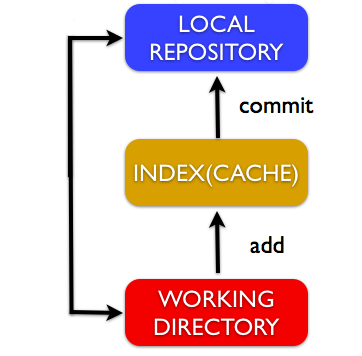
\includegraphics[width=1.5in]{images/data_flow_simplified.png}
         \end{figure}
   \end{columns}
}

\frame{
   \frametitle{The problem}
   \begin{figure}
      \centering
      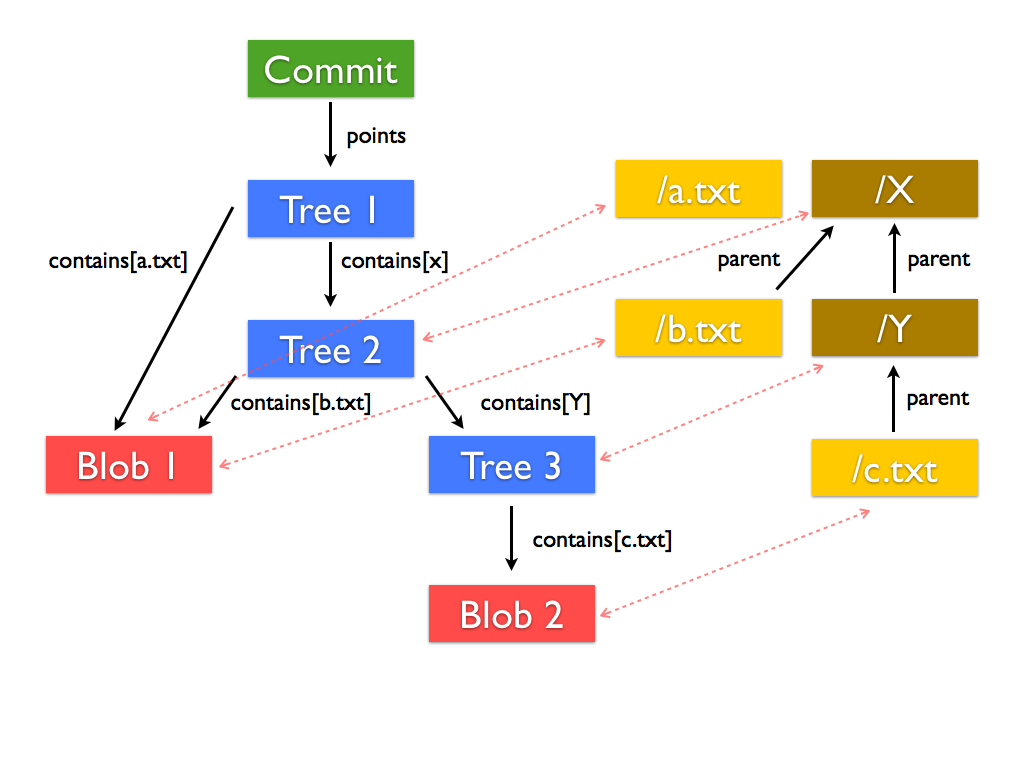
\includegraphics[width=0.9\textwidth]{images/structures.png}
   \end{figure}
}
\section{Progress}
\begin{frame}[fragile]
   \frametitle{How did we solve it?}
   \begin{columns}[c]
      \column{2.5in}
         \begin{block}{Abstraction}
            \begin{itemize}
               \item In each commit there is relation between Objects and Paths
               \item Facts to reflect the parent relationship
         \end{itemize}
         \end{block}
      \column{1.5in}\\


      \tiny
      \begin{lstlisting}[escapechar=!]
sig Commit extends Object {
   points : Tree,
   parent : set Commit,
   !\color{red}{abs: Path -> Object}!
}
     \end{lstlisting}
   \end{columns}
   \tiny
   \begin{lstlisting}[escapechar=!]
         all c: Commit{
            let objs = c.points.*(contents.Name){
               c.abs in Path some -> lone objs
               (c.abs).(c.points) in Root
               all p,q : (c.abs).univ | p -> q in pathparent 
                  implies q.(c.abs) -> p.(c.abs) -> p.name in contents
               all t,o : objs, n : Name | t -> o -> n in contents 
                  implies all y : c.abs.t | some x : c.abs.o | 
                     x -> y in pathparent and x.name = n
            }
         }
   \end{lstlisting}  
\end{frame}

\frame{
   \frametitle{The abstraction relation}
   \begin{figure}
      \centering
      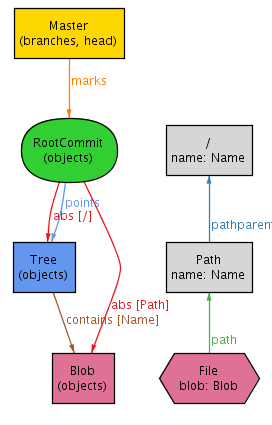
\includegraphics[width=0.3\textwidth]{images/abs1.png}
   \end{figure}

}

\frame{
   \frametitle{The abstraction relation}
   \begin{figure}
      \centering
      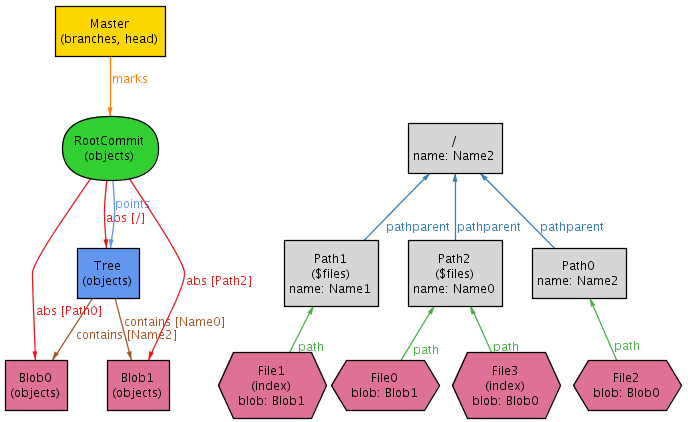
\includegraphics[width=0.8\textwidth]{images/abs2.png}
   \end{figure}

}

\section{Current Model}
\begin{frame}[fragile]
   \frametitle{Model}
   \tiny
   \begin{columns}[c]
      \column{1.5in}
         \begin{lstlisting}
abstract sig Object {
   objects: set State
}

sig Blob extends Object {}

sig Tree extends Object {
   contains : Name -> lone (Tree+Blob)
}

sig Commit extends Object {
   points : Tree,
   parent : set Commit,
   abs: Path -> Object
}

sig RootCommit extends Commit {}

sig Branch{
   marks: Commit one -> State,
   branches: set State,
   head: set State
}

lone sig Master extends Branch{}
                  
         \end{lstlisting}
      \column{1.5in}
      \color{blue}{
         \begin{lstlisting}
sig Path {
   pathparent : lone Path,
   name : Name
}

sig File{
   path: Path,
   blob: Blob,
   index: set State
}
         \end{lstlisting}
      }
   \end{columns}
\end{frame}


\section{The operations}
\begin{frame}[fragile]
   \frametitle{Operations - add and rm}
   \begin{block}{add}
      Add a file with the current content to the index.
   \end{block}
   \tiny
   \begin{lstlisting}
...
index.s' = index.s + 
           f - ((f.path).~path -f)
...   
   \end{lstlisting}
   \normalsize
   \begin{block}{rm}
      Remove the file from index.
   \end{block}
   \tiny
   \begin{lstlisting}
...
index.s' = index.s - f
...
   \end{lstlisting}
\end{frame}

\begin{frame}[fragile]
   \frametitle{Operations - add and rm}
   \begin{figure}
      \centering
      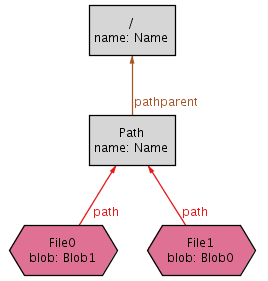
\includegraphics[width=0.4\textwidth]{images/add1.png}
   \end{figure}
\end{frame}

\begin{frame}[fragile]
   \frametitle{Operations - add and rm}
   \begin{figure}
      \centering
      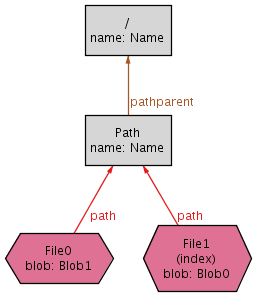
\includegraphics[width=0.4\textwidth]{images/add2.png}
   \end{figure}
\end{frame}

\begin{frame}[fragile]
   \frametitle{Operations - commit}
   \begin{block}{commit}
      Creates a commit, from the index.
   \end{block}
   \tiny
   \begin{lstlisting}
...
(head.s').(marks.s').parent = (head.s).(marks.s)
...
(index.s).path.*pathparent = (head.s').(marks.s').abs.univ
all f:index.s | f.path -> f.blob in (head.s').(marks.s').abs
...
   \end{lstlisting}
\end{frame}

\begin{frame}[fragile]
   \frametitle{Operations - commit}
   \begin{figure}
      \centering
      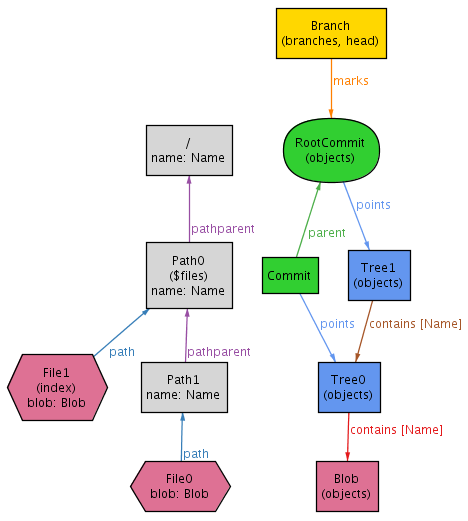
\includegraphics[width=0.5\textwidth]{images/commit1.png}
   \end{figure}
\end{frame}

\begin{frame}[fragile]
   \frametitle{Operations - commit}
   \begin{figure}
      \centering
      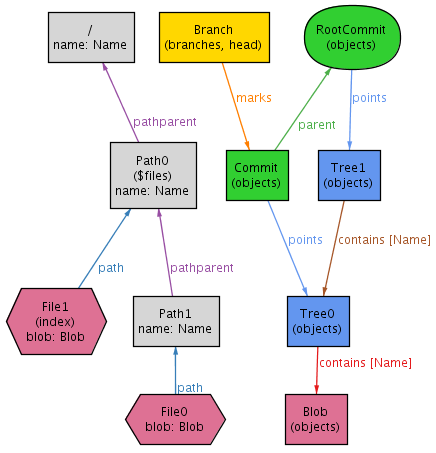
\includegraphics[width=0.5\textwidth]{images/commit2.png}
   \end{figure}
\end{frame}

\begin{frame}[fragile]
   \frametitle{Operations - branch}
   \begin{block}{branch}
      Creates a new branch pointing to the current one.
   \end{block}
   \tiny
   \begin{lstlisting}
...
branches.s' = branches.s + b
marks.s' = marks.s + b -> (head.s).(marks.s)
...
   \end{lstlisting}
   \normalsize
   \begin{block}{branch -d}
      Removes a branch if it is not pointed by the head.
   \end{block}
   \tiny
   \begin{lstlisting}
...
branches.s' = branches.s - b
marks.s' = marks.s - b -> Commit
...
   \end{lstlisting}
\end{frame}

\begin{frame}[fragile]
   \frametitle{Operations - branch}
   \begin{columns}[c]
      \column{1.5in}
      \begin{figure}
         \centering
         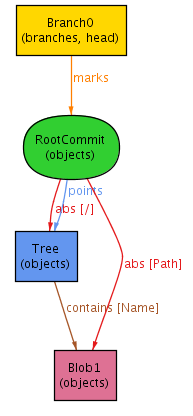
\includegraphics[width=0.75\textwidth]{images/branch1.png}
      \end{figure}
      \pause
      \column{1.5in}
      \begin{figure}
         \centering
         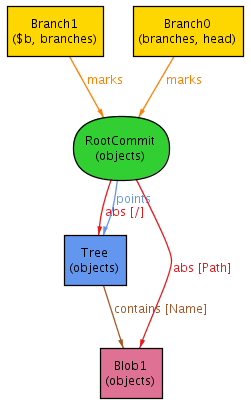
\includegraphics[width=0.90\textwidth]{images/branch2.png}
      \end{figure}
   \end{columns}
\end{frame}

\begin{frame}[fragile]
   \frametitle{Operations - branch}
\end{frame}

\begin{frame}[fragile]
   \frametitle{Operations - checkout}
   \begin{block}{checkout}
      Updates the index to reflect a certain commit pointed by a
      branch.
   \end{block}
\end{frame}

\section{The properties}
\frame{
   \frametitle{Properties}
}
\section{Future work}
\frame{
   \frametitle{Future work}
}

\frame{
   \titlepage
}


\end{document}
